\section{Experiments and analysis}\label{sec:evaluation}
\subsection{Workload, splits and service contract}
The controlled workload uses native SUMO mobility~\cite{sumo}, a versioned directed
road graph derived from public geographic inputs, and 418 POIs in six categories
with OpenStreetMap provenance~\cite{osm}. The graph contains 66,189 road states,
4,849 external edges and 21,179 internal edges. The compiled native network is
not asserted to reproduce every original Beijing lane or junction.

The source cohort has 48 route families. The experiment retains days 7 and 8
and a 600-second window with 31 service ticks at 20-second spacing. Families
are disjoint across 20 TRAIN, 8 SELECTION and 20 TEST groups. TRAIN/SELECTION
use one retained draw per native trip; TEST uses three, giving 120 trip-draws
per arm from 40 test trips. Repeated draws are not independent route families.
Eligibility uses declared road geometry and route-calibration rules rather
than defense protection scores. This cohort and map were inspected during
development; the study is not a fresh-city or untouched-geometry confirmation.

All arms use the same catalogue, $L=60$ per category/coordinate, local filters,
reference costs and tie-breaking. The four purposes minimize road distance,
minimize travel time, filter within 1,000 m and rank by distance, or minimize
detour to a private local destination. A reference contains up to five items.
The application answer itself is not truncated to five. Empty references remain
not applicable (N/A), with their denominators retained.

We distinguish current-packet, 60-second epoch and whole-session caches.
The principal utility result uses a static session cache. The provider's
complete reply signatures are public design resources and match the
experimental provider. This controlled condition is essential to interpreting
the high coverage and does not establish a need for repeated remote acquisition.

\subsection{Comparisons and attack protocol}
\begingroup\footnotesize
\begin{longtable}{@{}P{2.7cm}P{3.6cm}P{7.3cm}@{}}
\caption{Controls, adaptations and the frozen proposed method.}\label{tab:methods}\\
\toprule\textbf{Method} & \textbf{Public output contract} & \textbf{Configuration / fidelity} \\
\midrule\endfirsthead
\multicolumn{3}{l}{\textit{Continued from previous page}}\\
\toprule\textbf{Method} & \textbf{Public output contract} & \textbf{Configuration / fidelity} \\
\midrule\endhead
\midrule\multicolumn{3}{r}{\textit{Continued on next page}}\\\endfoot
\bottomrule\endlastfoot
Raw GPS & One real coordinate & Unprotected control \\
REM-Z (K1) & One REM coordinate & $u=0.01\,\mathrm m^{-1}$; frozen references \\
TransProtect* & One replacement coordinate & Markov predictor; $K=10$, 8 TRAIN targets, $\alpha_{\rm TP}=10000$, $\varepsilon=0.005\,\mathrm m^{-1}$ \\
Semantic* & True point + 4 dummies & OSM/empirical predictor; candidate pool 128; replaces AMap/LSTM \\
Fake queries* & K5 sets + inserted fake events & Road/history predictor; up to 2 fake events, waits 5--15 s, 24 candidates, similarity 0.75 \\
\textbf{GeoI-BQ v1} & K5 committed frames & $\Gamma_Q=1$, $C_s=0.23\,\mathrm m^{-1}$; protected read interval $\ge60$ s \\
\end{longtable}
The methods have different guarantees, output cardinalities and costs. We do not equate their epsilon values.
\endgroup

Table~\ref{tab:methods} lists six implementations. The three starred methods
are audited adaptations with declared substitutions, not official author
reproductions or matched-privacy-budget executions. GeoI-BQ and direct REM-Z
replay their frozen coordinates and timestamps without favorable resampling.
Fake-query insertion retains all naturally emitted extra packets.

The attack bank includes geometry/history estimators, ExtraTrees with 64
trees~\cite{extratrees}, shadow kNN-1/kNN-5 and priors. Endpoint tasks add
ordered and geometry-linked sequences. Models fit TRAIN; robust selection on
SELECTION is separate for each method, task and loss, using mean plus standard
error for MAE and mean minus standard error for Hit. TEST never supplies
estimator features, true-member flags, internal $Z$, belief or evaluator indices.
Hit and MAE in the same cell may therefore come from different selected estimators.
For GeoI-BQ, the principal Hit100 selector chooses centroid in all five tasks;
MAE selects prior-based estimators. This is not evidence that a Bayes-optimal
attacker failed.

S1 observes one packet at a service tick. S2 observes all wire from 540 to
600 seconds and targets the mean of four final GPS ticks, a coordinate proxy
rather than semantic home/work inference. S3 uses the complete 0--600-second
wire to reconstruct the 31 target positions. S9 and S10 estimate the first
and last GPS from the full wire with known public boundaries. Comparisons use
the same time window, not the same number of packets; auxiliary fake events
remain visible and are charged.

For error $e_i=\|x_i-\widehat x_i\|_2$, the principal privacy metrics are
$\operatorname{Hit100}=N^{-1}\sum_i\mathbf1_{\{e_i\le100\}}$ and
$\operatorname{MAE}=N^{-1}\sum_i e_i$. Lower Hit and higher MAE favor protection
within the declared task. S3 Hit is pointwise reconstruction performance
aggregated over time, not a whole-route success probability. Utility uses
(\ref{eq:recall}) and equal-purpose macro averaging over defined references.
Values aggregate within trip, then family, then across test families.
We use 10,000 paired family bootstrap replicates for 95\% percentile
intervals~\cite{efron}. Intervals condition on the retained cohort and models;
they do not capture all dataset-generation, selection or domain-shift uncertainty.
Failures retain coverage and are not counted as successful privacy.

\subsection{Localization, utility and cost}
\begin{table}[htbp]\centering\footnotesize
\caption{Localization results: Hit100 (\%, lower) / MAE (m, higher). Same time windows.}\label{tab:privacy}
\begin{tabularx}{\linewidth}{@{}P{2.7cm}YYYYY@{}}\toprule
\textbf{Method} & \textbf{S1} & \textbf{S2} & \textbf{S3} & \textbf{S9} & \textbf{S10} \\
\midrule
Raw GPS & \shortstack[l]{100.000 /\\ 0.0} & \shortstack[l]{100.000 /\\ 0.0} & \shortstack[l]{100.000 /\\ 0.0} & \shortstack[l]{100.000 /\\ 0.0} & \shortstack[l]{100.000 /\\ 0.0} \\
REM-Z (K1) & \shortstack[l]{18.522 /\\ 338.5} & \shortstack[l]{37.500 /\\ 214.3} & \shortstack[l]{18.522 /\\ 338.5} & \shortstack[l]{5.833 /\\ 435.8} & \shortstack[l]{35.000 /\\ 246.8} \\
TransProtect* & \shortstack[l]{82.984 /\\ 54.4} & \shortstack[l]{94.167 /\\ 28.7} & \shortstack[l]{82.984 /\\ 54.4} & \shortstack[l]{96.667 /\\ 17.8} & \shortstack[l]{90.833 /\\ 33.6} \\
Semantic* & \shortstack[l]{82.258 /\\ 41.9} & \shortstack[l]{100.000 /\\ 8.2} & \shortstack[l]{82.258 /\\ 41.9} & \shortstack[l]{100.000 /\\ 5.3} & \shortstack[l]{100.000 /\\ 7.3} \\
Fake queries* & \shortstack[l]{53.387 /\\ 1213.0} & \shortstack[l]{92.500 /\\ 239.1} & \shortstack[l]{98.790 /\\ 13.3} & \shortstack[l]{99.167 /\\ 42.2} & \shortstack[l]{100.000 /\\ 6.4} \\
\textbf{GeoI-BQ v1} & \shortstack[l]{0.188 /\\ 2104.6} & \shortstack[l]{0.000 /\\ 2124.2} & \shortstack[l]{0.188 /\\ 2104.6} & \shortstack[l]{0.000 /\\ 1986.4} & \shortstack[l]{0.000 /\\ 2124.2} \\
\bottomrule\end{tabularx}
\par\smallskip\raggedright * Audited adaptations, not official author implementations. Each loss has its own selected attacker. Full CIs appear in the supplement.
\end{table}

Table~\ref{tab:privacy} reports the five principal tasks. Raw recovers every
coordinate target with Hit100 100\%, establishing that the evaluation exposes
directly observed coordinates. GeoI-BQ has Hit100 0--0.188\% and MAE
1.99--2.12 km in the selected bank. Direct REM-Z remains more identifiable,
with Hit100 5.833--37.500\%.

The contrast with Fake-query insertion is instructive. Its S1 MAE is
1,213 m while Hit100 is still 53.387\%; with the whole S3 window,
Hit100 rises to 98.790\% and MAE falls to 13.3 m.
Additional fake events do not prevent a history-aware observer from exploiting
the known service clock in this adaptation. GeoI-BQ instead releases Q-only
actions from a broadly supported public library with bounded private tilting.
These are observations about the retained implementations, not universal
rankings of the original papers.

Zero-hit observations and degenerate bootstrap intervals do not imply zero
population risk. A large MAE also reflects the prior ambiguity and public
library geometry in this cohort; it is not a guaranteed noise displacement.
Full confidence intervals and selected estimators are supplied in the supplement.

\begin{table*}[t]\centering\footnotesize
\caption{Session-cache Recall@5 (\%, higher). The application returns a full sorted list.}\label{tab:utility}
\begin{tabularx}{\linewidth}{@{}P{2.7cm}YYYYY@{}}\toprule
\textbf{Method} & \textbf{Macro} & \textbf{Nearest} & \textbf{Fastest} & \textbf{Radius} & \textbf{Detour} \\
\midrule
Raw GPS & 99.999 & 100.000 & 100.000 & 100.000 & 99.995 \\
REM-Z (K1) & 99.700 & 99.753 & 99.753 & 99.625 & 99.668 \\
TransProtect* & 99.996 & 100.000 & 100.000 & 100.000 & 99.986 \\
Semantic* & 99.999 & 100.000 & 100.000 & 100.000 & 99.997 \\
Fake queries* & 99.999 & 100.000 & 100.000 & 100.000 & 99.997 \\
\textbf{GeoI-BQ v1} & 99.595 & 99.638 & 99.641 & 99.388 & 99.712 \\
\bottomrule\end{tabularx}
\end{table*}

GeoI-BQ achieves macro Recall 99.595\%, CI95\% [99.224, 99.903]\%.
It is approximately 0.4 percentage points below the three adaptations.
Against TransProtect*, the paired difference is $-0.401$ percentage points,
CI95\% [$-0.773$, $-0.093$]. Radius is the most sensitive purpose.
We retain the adverse sign and do not claim utility superiority.

\begingroup\footnotesize
\begin{longtable}{@{}P{2.7cm}P{2.2cm}P{2.2cm}P{2.2cm}P{2.2cm}@{}}
\caption{Mean wire cost per 600-second session; KB denotes 1,000 bytes.}\label{tab:cost}\\
\toprule\textbf{Method} & \textbf{Packets} & \textbf{Coordinates} & \textbf{Request KB} & \textbf{Reply KB} \\
\midrule\endfirsthead
\multicolumn{5}{l}{\textit{Continued from previous page}}\\
\toprule\textbf{Method} & \textbf{Packets} & \textbf{Coordinates} & \textbf{Request KB} & \textbf{Reply KB} \\
\midrule\endhead
\midrule\multicolumn{5}{r}{\textit{Continued on next page}}\\\endfoot
\bottomrule\endlastfoot
Raw GPS & 31.00 & 31.00 & 5.846 & 16.843 \\
REM-Z (K1) & 31.00 & 31.00 & 6.352 & 16.921 \\
TransProtect* & 31.00 & 31.00 & 6.351 & 16.847 \\
Semantic* & 31.00 & 155.00 & 31.754 & 84.770 \\
Fake queries* & 38.04 & 190.21 & 39.418 & 104.033 \\
\textbf{GeoI-BQ v1} & 31.00 & 155.00 & 31.756 & 82.557 \\
\end{longtable}
Request/reply serialization is the replay contract; reply bytes encode POI indices, not full production records, TLS or network energy.
\endgroup

Each 600-second session uses 155 coordinate queries for GeoI-BQ, compared with
31 for singleton controls and TransProtect*, 155 for Semantic*, and about
190.21 for Fake-query insertion*. The last arm emits approximately 38.04
packets rather than 31. Byte measurements serialize request/reply-index JSON:
they exclude full POI metadata, HTTP/TLS, radio latency and energy.
Generation timing for replayed GeoI-BQ and REM-Z is unavailable in this trial.
Shared service replay timings are not comparable device latency measurements.

\begin{figure}[htbp]\centering
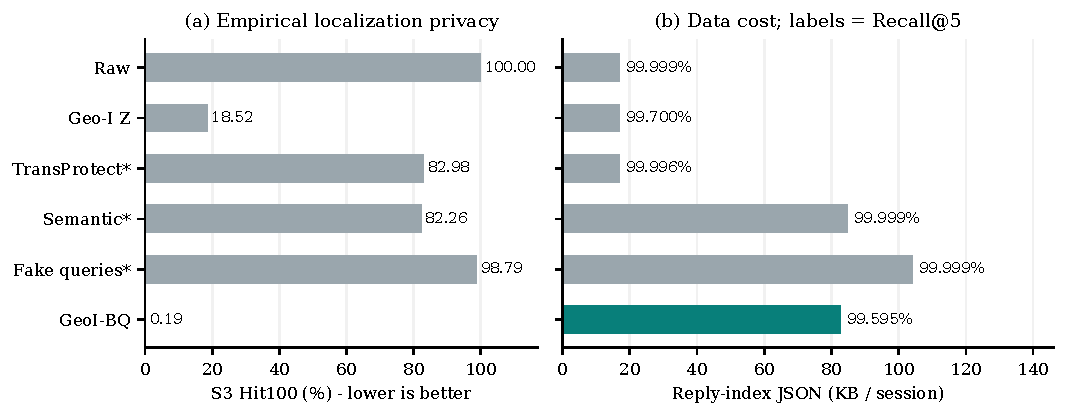
\includegraphics[width=\linewidth]{figure_tradeoff.pdf}
\caption{Controlled privacy--utility--cost comparison. Left: S3 Hit100
(lower favors protection). Right: reply-index JSON cost, with session
Recall labels. Starred methods are adaptations; neither equal cost nor
equal formal privacy is assumed.}\label{fig:tradeoff}
\end{figure}

\subsection{Original metrics and supplementary inference tasks}
The original-metric comparison is partial. The S3 point-error measure has
the expected-distance form of EIE, but does not reproduce TransProtect's
VehiTrack attack. For singleton outputs, its Equation-13 travel-cost
distortion is evaluated with eight TRAIN-selected targets/prior and directed
road distances: TransProtect* yields 47.44 m and REM-Z 688.65 m.
This is a local-target proxy, not experimental parity with the original
Rome/San Francisco study. GeoI-BQ has no unique released singleton to use
in that expression; selecting a secret-nearest Q would be invalid.
Real-member ASR, dummy-effectiveness DER and source-compatible path counts
remain unavailable or inapplicable for explicitly different reasons.
The supplement separates original metrics, task-aligned proxies, missing
reproduction inputs and incompatible contracts.

\begin{table*}[t]\centering\footnotesize
\caption{Extended diagnostics (\%); lower inference is preferable, subject to task validity.}\label{tab:scenario-summary}
\begin{tabularx}{\linewidth}{@{}P{2.7cm}YYY@{}}\toprule
\textbf{Method} & \textbf{S4 balanced acc.} & \textbf{S6 post-turn acc.} & \textbf{S8 protected-partner Hit100} \\
\midrule
Raw GPS & 100.00 & 100.00 & 100.00 \\
REM-Z (K1) & 91.67 & 50.00 & 6.67 \\
TransProtect* & 99.17 & 95.00 & 64.17 \\
Semantic* & 100.00 & 95.00 & 75.00 \\
Fake queries* & 93.33 & 99.17 & 68.33 \\
\textbf{GeoI-BQ v1} & 47.50 & 50.83 & 0.00 \\
\bottomrule\end{tabularx}
\par\smallskip\raggedright S4 is route-family association, not verified person/vehicle identity. S6 has two candidates (50\% chance). S8 is the post-V1 fusion diagnostic on the inspected cohort.
\end{table*}

Table~\ref{tab:scenario-summary} summarizes additional tasks; full six-arm
results are in the supplement. S4 is balanced route-family association,
not physical person/vehicle re-identification. GeoI-BQ's balanced accuracy
is 47.50\%, CI95\% [40.00, 54.17]\%. S5's Raw accuracy is 50\%:
the cadence misses informative turn observations, so its chance-level defense
score cannot establish a protection contribution. S6's post-turn two-destination
task is more informative: Raw achieves 100\%, adaptations 95--99.17\%,
and GeoI-BQ 50.83\%, CI95\% [44.17, 57.50]\%. REM-Z also achieves 50\%,
so this does not isolate a benefit from the Q layer.

S7 changes four purposes and six categories at fixed trajectory/context.
All 1,056 streams have equal wire across 25,344 counterfactuals. The joint
conditional Bayes vulnerability is $1/24$ under the balanced test prior.
All arms share this cover wrapper; it is not a unique advantage over the
papers' original interfaces or a natural-intent attack result.

S8 aligns two correlated synthetic native prefixes, grants channel association,
and evaluates target-only, protected-partner, Raw-partner and unrelated-partner
views. A stronger post-readout fusion bank increases Semantic* Hit100 from
45\% to 75\% and Fake-query* from 16.67\% to 68.33\%; GeoI-BQ has no hits
in the retained protected-partner sample. With a perfectly aligned Raw partner,
an available direct estimator attains 100\% in every arm. This is a diagnostic
of strong side information, not native simultaneous co-travel or independent
confirmation. The weaker bank and initial verifier-gate failure remain preserved.

\subsection{Attribution and limits of the application claim}
High Recall is explained partly by the small static catalogue and response
depth. Five coordinates times six categories times $L60$ permit up to
1,800 reply entries before deduplication against only 418 POIs.
A read-only audit of all 120 retained TEST draws finds 380.2 unique POIs
in the first GeoI-BQ packet on average (range 379--383), and 415.875 in the
final session cache (403--418): approximately 91\% and 99.49\% of the catalogue.
Current-packet Recall is 96.780\%, epoch-cache Recall 97.123\%, and
session-cache Recall 99.595\%. This is evidence of effective acquisition
and cache use under the contract, but weakly discriminates private planning
from broad public cover.

The matched public base $\Gamma_Q=0$ achieves 99.711\% Recall, exceeding
the primary policy by about 0.116 percentage points; the original paired
interval for primary minus base is [$-0.253$, $-0.006$] percentage points.
This supports the unfavorable direction in the observed cohort, not universal
dominance. It also agrees with (\ref{eq:gain}): score gain alone is insufficient.
We retain the policy family and its accounting without declaring private
adaptation necessary or optimal.

The data-access audit is stronger than a hypothetical bulk-API objection:
the prototype itself loads complete reference data sufficient for the four
static objectives. Therefore online necessity is not established against a
client allowed to use that information directly. A deployment must distinguish
offline design resources from genuinely unavailable current metadata and
measure acquisition/setup/refresh costs for an equally informed control.
The current offline-information result is analytical, not a measured seventh
arm with zero total system cost.

Duration is another untested regime. At most 11 protected reads fit the
0--600-second clock; worst-case spend is $1+2(11-1)=21<23$ units.
All retained ledgers end at 13--21 units, with no cap exhaustion.
The duration-independent privacy accounting consequently has not been
paired with an empirical utility test after new protected GPS is disallowed.

Finally, the theory is conditional on common support, fixed/public boundary
rules, provider laws and valid state handling. Integer Q sampling does not
certify floating-point REM, practical entropy or full upstream restoration.
Physical identity, correlated intent, user feedback and linked sessions
require their own conditions. These limitations constrain the interpretation
of the results; they are not erased by low empirical Hit100.
